\PassOptionsToPackage{unicode=true}{hyperref} % options for packages loaded elsewhere
\PassOptionsToPackage{hyphens}{url}
%
\documentclass[
  12pt,
]{article}
\usepackage{lmodern}
\usepackage{amssymb,amsmath}
\usepackage{ifxetex,ifluatex}
\ifnum 0\ifxetex 1\fi\ifluatex 1\fi=0 % if pdftex
  \usepackage[T1]{fontenc}
  \usepackage[utf8]{inputenc}
  \usepackage{textcomp} % provides euro and other symbols
\else % if luatex or xelatex
  \usepackage{unicode-math}
  \defaultfontfeatures{Scale=MatchLowercase}
  \defaultfontfeatures[\rmfamily]{Ligatures=TeX,Scale=1}
  \setmainfont[]{Times New Roman}
\fi
% use upquote if available, for straight quotes in verbatim environments
\IfFileExists{upquote.sty}{\usepackage{upquote}}{}
\IfFileExists{microtype.sty}{% use microtype if available
  \usepackage[]{microtype}
  \UseMicrotypeSet[protrusion]{basicmath} % disable protrusion for tt fonts
}{}
\makeatletter
\@ifundefined{KOMAClassName}{% if non-KOMA class
  \IfFileExists{parskip.sty}{%
    \usepackage{parskip}
  }{% else
    \setlength{\parindent}{0pt}
    \setlength{\parskip}{6pt plus 2pt minus 1pt}}
}{% if KOMA class
  \KOMAoptions{parskip=half}}
\makeatother
\usepackage{xcolor}
\IfFileExists{xurl.sty}{\usepackage{xurl}}{} % add URL line breaks if available
\IfFileExists{bookmark.sty}{\usepackage{bookmark}}{\usepackage{hyperref}}
\hypersetup{
  pdftitle={State-Space Model to Estimate Salmon Escapement Using Multiple Data Sources},
  pdfauthor={Kevin E. See1,, Ryan N. Kinzer2, and Mike W. Ackerman1},
  pdfkeywords={escapement; Chinook; steelhead; Lower Granite Dam; state-space model; Bayesian model},
  pdfborder={0 0 0},
  breaklinks=true}
\urlstyle{same}  % don't use monospace font for urls
\usepackage[margin=1in]{geometry}
\usepackage{longtable,booktabs}
% Allow footnotes in longtable head/foot
\IfFileExists{footnotehyper.sty}{\usepackage{footnotehyper}}{\usepackage{footnote}}
\makesavenoteenv{longtable}
\usepackage{graphicx,grffile}
\makeatletter
\def\maxwidth{\ifdim\Gin@nat@width>\linewidth\linewidth\else\Gin@nat@width\fi}
\def\maxheight{\ifdim\Gin@nat@height>\textheight\textheight\else\Gin@nat@height\fi}
\makeatother
% Scale images if necessary, so that they will not overflow the page
% margins by default, and it is still possible to overwrite the defaults
% using explicit options in \includegraphics[width, height, ...]{}
\setkeys{Gin}{width=\maxwidth,height=\maxheight,keepaspectratio}
\setlength{\emergencystretch}{3em}  % prevent overfull lines
\providecommand{\tightlist}{%
  \setlength{\itemsep}{0pt}\setlength{\parskip}{0pt}}
\setcounter{secnumdepth}{-2}
% Redefines (sub)paragraphs to behave more like sections
\ifx\paragraph\undefined\else
  \let\oldparagraph\paragraph
  \renewcommand{\paragraph}[1]{\oldparagraph{#1}\mbox{}}
\fi
\ifx\subparagraph\undefined\else
  \let\oldsubparagraph\subparagraph
  \renewcommand{\subparagraph}[1]{\oldsubparagraph{#1}\mbox{}}
\fi

% set default figure placement to htbp
\makeatletter
\def\fps@figure{htbp}
\makeatother

% double spacing
\usepackage{setspace}
\doublespacing
% to double space figure captions
\usepackage{caption}
\captionsetup{font = doublespacing}

% line numbers
\usepackage{lineno}
\linenumbers
\usepackage{booktabs}
\usepackage{longtable}
\usepackage{array}
\usepackage{multirow}
\usepackage{wrapfig}
\usepackage{float}
\usepackage{colortbl}
\usepackage{pdflscape}
\usepackage{tabu}
\usepackage{threeparttable}
\usepackage{threeparttablex}
\usepackage[normalem]{ulem}
\usepackage{makecell}
\usepackage{xcolor}

\title{State-Space Model to Estimate Salmon Escapement Using Multiple Data Sources}
\author{Kevin E. See\textsuperscript{1,*}, Ryan N. Kinzer\textsuperscript{2}, and Mike W. Ackerman\textsuperscript{1}}
\date{August 18, 2020}

\begin{document}
\maketitle
\begin{abstract}
This is the abstract
\end{abstract}

\textsuperscript{1} Biomark, Inc.~705 South 8th St., Boise, Idaho, 83702, USA\\
\textsuperscript{2} Nez Perce Tribe, Department of Fisheries Resource Management, 14054 Burr Road, PO Box 1942, McCall, Idaho, 83638, USA

\textsuperscript{*} Correspondence: \href{mailto:Kevin.See@merck.com}{Kevin E. See \textless{}\href{mailto:Kevin.See@merck.com}{\nolinkurl{Kevin.See@merck.com}}\textgreater{}}

\textbf{Possible journals:}

First Choice:

\begin{itemize}
\tightlist
\item
  \textbf{\href{https://afspubs.onlinelibrary.wiley.com/journal/15488675}{North American Journal of Fisheries Management}}
\end{itemize}

Second Choice:

\begin{itemize}
\tightlist
\item
  \href{https://afspubs.onlinelibrary.wiley.com/journal/15488659}{Transactions of the American Fisheries Society}
\end{itemize}

Others:

\begin{itemize}
\item
  \href{http://www.nrcresearchpress.com/page/cjfas/editors}{Canadian Journal of Fisheries and Aquatic Sciences}
\item
  \href{https://www.journals.elsevier.com/fisheries-research}{Fisheries Research}
\item
  \href{http://fishbull.noaa.gov/}{Fishery Bulletin}
\item
  \href{http://onlinelibrary.wiley.com/journal/10.1111/(ISSN)1467-2979/homepage/ProductInformation.html}{Fish and Fisheries}
\end{itemize}

\hypertarget{introduction}{%
\section{Introduction}\label{introduction}}

Fish escapement is the number of adults that survive juvenile and adult rearing, escape harvest and return to their natal habitat to potentially spawn (e.g.~Bue et al. (1998)). For anadromous fishes, escapement is often estimated at a fixed location in a river system prior to fish reaching their spawning area. Escapement estimates facilitate effective fisheries management, and particularly, estimates of escapement for each component group (e.g., stock, population, age, origin {[}wild, hatchery{]}; Hess et al. (2014); Steinhorst et al. (2017)) provide valuable information that fisheries managers use to achieve sustainable harvest, while protecting small and vulnerable populations. Accurate escapement estimates are increasingly important for depleted populations as they inform viable salmonid metrics (McElhany et al. 2000), and facilitate assessments of population viability and extinction risk (Ford et al. 2015; Williams et al. 2016) and climate change vulerability (Crozier et al. 2019).

Populations of Chinook Salmon Oncorhynchus tshawytscha and steelhead trout O. mykiss in the Snake River basin of Pacific Northwest, USA, are depleted following decades of substantial harvest and anthropogenic changes to their migration corridor (e.g., construction of hydroelectric dams on the Snake and Columbia rivers) and tributary habitats (Nehlsen et al. 1991; McClure et al. 2003; Ford et al. 2015). As a result, Snake River spring-summer run Chinook Salmon (hereafter Chinook Salmon) were classified as threatened in 1992 under the Endangered Species Act (ESA; Federal Registry Notice 57 FR 14653), and Snake River summer-run steelhead trout (hereafter steelhead) were listed as threatened five years later (Federal Registry Notice 62 FR 43937). Snake River Chinook Salmon and steelhead have substantial recreational, commercial, cultural and subsistence value both within the Snake River basin as well as in downstream corridors (i.e., Columbia River) and ocean fisheries. The aggregate escapement of Snake River Chinook Salmon and steelhead populations, with the exception of Tucannon River, is measured at Lower Granite Dam located in southeast Washington; the final dam on the Snake River that returning adults must pass prior to heading to tributary spawning locations. Many fisheries management and conservation actions are made based on estimates of escapement at Lower Granite Dam parsed by species and origin (\textbf{Snake Basin Harvest Plans?}). Additionally, harvest openings and closures, both upstream in Snake River fisheries and downstream in mainstem Snake and Columbia River fisheries, are predicated on escapements at Lower Granite Dam (\textbf{could cite US v OR Management Agreement and Snake Basin Harvest Plans?}).

Chinook Salmon and steelhead returning to a majority of populations in the Snake River must ascend a fish ladder on Lower Granite Dam before migrating to their natal tributary spawning locations. Fish management agencies previously used counts of fish, by species, passing an observation window located on the side of the fish ladder as a census of fish escaping past the dam. For both species, total escapement was then parsed into groups (e.g., wild, hatchery) using observed marks and genetic data from a sample of fish captured at an adult trap located on the fish ladder upstream of the observation window (Camacho et al. 2017 p. @Steinhorst2017). Window counts as a census proved beneficial as being an easy, straight-forward method that was ascertained in near real-time. Moreover, downriver fisheries management arenas have used window counts at lower-river dams as escapement estimates for the past several years, and consistency in methods is often desirable for management decision making (\textbf{citation?}).

Using window counts, however, as a census of Chinook Salmon and steelhead passing Lower Granite Dam can be problematic as it avoids multiple sources of uncertainty and ignores known biological processes. First, live (i.e., in-person) window counts only occur from April through October each year. Additionally, live window counts only occur for 16-hours each day, and fish counters working at the observation window look directly into the fish ladders to identify and count all passing fish, by species, for only 50 minutes of each hour. Counts are then expanded to provide an estimate for the hour (USACE 2015). From November through March, the remainder of the year, video tape fish counting is used and only occurs for 10 hours each day; fish counters then read the video tapes and submit daily fish counts (Hatch et al. 1994). Typically, the observational error rates of live and video window counts are unknown, and sampling error rates are ignored. Additionally, two biological processes are unaccounted for: 1) fish that cross the dam during the 8-hours when the window is closed for counting (i.e., nighttime passage) which may result in an underestimate of escapement, and 2) fish that cross the dam multiple times (i.e., re-ascension), and therefore potentially double-counted. Finally, Chinook Salmon and steelhead that migrate through the ladder and past the dam may fallback over the dam (e.g., over spillway, through navigation locks), and later, may or may not re-ascend the fish ladder again (Boggs et al. 2004). Both fallback with no re-ascension and fallback with re-ascension potentially result in an overestimate of escapement (Dauble and Mueller 2000). Previously, it was assumed that nighttime passage rates and fallback/re-ascension rates cancelled each other out resulting in window counts providing an unbiased estimate of escapement (\textbf{citation?})

In this study, we describe a novel method to estimate aggregate and group escapement which incorporates all sources of known uncertainty, we demonstrate the estimation method is essentially unbiased, thus improving effective conservation and management decision making, and show night-time passage and fallback/re-ascension rates are unequal. Our method for estimating escapement, by species, past Lower Granite Dam incorporates window counts, data from the adult fish trap, and observations of PIT tagged fish in the adult ladder to explicitly model nighttime passage, re-ascension, and error from both window and trap estimates using a state-space approach (Royle and Dorazio 2008). To meet desired management and conservation objectives, modeled escapement includes estimates of uncertainty and is parsed into weekly strata. Further, total and weekly estimates are parsed into three origin groups: wild, hatchery, and hatchery no-clip. Estimates of escapement account for fish that migrate through the ladder at night outside of observation hours and account for fish that may ascend the ladder multiple times due to fallback and re-ascension. Our model is implemented in the \textbf{ST}ate-space \textbf{A}dult \textbf{D}am \textbf{E}scapement \textbf{M}odel (STADEM) package for the statistical software R (R Core Team 2020), and is available for downloaded at \url{https://github.com/KevinSee/STADEM}. To validate the STADEM results, we simulated 12 scenarios with varying trapping rates, fallback and re-ascension rates, nighttime passage rates, and window count error rates. The STADEM model combines multiple imperfect sources of data to reduce bias in escapement estimates and provide more reasonable estimates of uncertainty. Additionally, the STADEM model framework can be applied elsewhere to estimate aggregate and group escapement, provided a passage barrier containing multiple counting and observational mechanisms exist, such as, a counting window, an adult trap sampling a portion of the run, and PIT tag antenna infrastructure.

\hypertarget{methods}{%
\section{Methods}\label{methods}}

\hypertarget{data-requirements}{%
\subsection{Data Requirements}\label{data-requirements}}

We used STADEM and three sources of data to estimate Chinook Salmon and steelhead escapement at Lower Granite Dam from 2010-2019. Data sources included 1) counts of fish migrating past the observation window located on the adult fish ladder at Lower Granite, 2) information from adults captured at a fish trap located in the fish ladder, and 3) observations of previously PIT tagged fish detected in the adult fish ladder. Following, we describe each of the data sources in more detail as they pertain to Lower Granite Dam; however, similar data could likely be obtained from other fish passage facilities.

\hypertarget{window-counts}{%
\subsubsection{Window Counts}\label{window-counts}}

Daily counts of adult Chinook Salmon and steelhead passing an observation window located on the Lower Granite fish ladder were the first source of data. Daily counts were made and provided by the US Army Corps of Engineers, and when summed, provide an estimate of the number of fish ascending and passing (i.e., escapement) Lower Granite Dam each season. Window counts were made for each species using video monitoring and direct in-person visual monitoring during daytime hours (Hatch et al. 1994). Video monitoring occured during the beginning and tail ends of the adult runs (March 1 -- March 31 and November 1 -- December) for 10 hours per day (0600 -- 1600 hours). Direct visual monitoring occured during peak run times (April 1 -- October 31) for 16 hours per day (0400 -- 2000 hours) (USACE 2015). During direct visual monitoring, observers recorded each adult (≥ 30cm), by species, passing the window for 50 minutes of each hour of operation. Salmonids under 30cm in length were not identified to species. The sum of the daily 50-minute counts were then multiplied by 1.2 to account for the 10 minutes when fish were not counted. Daytime window counts were not expanded for fish that may have ascended the ladder outside of operational hours (i.e., nighttime) (USACE 2015). Window counts were accessed through the Columbia Basin Research Data Access in Real Time (DART) website, \url{www.cbr.washington.edu/dart/query/adult_daily}, using their window count query. Counts were provided for each day the fish ladder was open to passage. Although window counts were assumed to be a census of every fish passing Lower Granite Dam, corrections were not applied for nighttime passage or re-ascending fish. Further, there was no estimation of daily or seasonal observation or sampling error.

\hypertarget{adult-fish-trap-data}{%
\subsubsection{Adult Fish Trap Data}\label{adult-fish-trap-data}}

The second source of data came from a sample of fish collected in the adult trap as they migrated past Lower Granite Dam (Ogden 2016a). The trap, also located within the adult fish ladder and upstream of the observation window, provided biological data (e.g., origin {[}wild, hatchery{]}, genetic stock, length, age, sex) for captured adults that allowed decomposition of the escapement into specific groups (e.g., Camacho et al. (2019), Steinhorst et al. (2017)). The trap was operational for 24 hours per day, and randomly sampled the daily run by opening four times per hour for a length of time determined by a set daily trapping rate. The trap rate was determined by a committee of collaborating management agencies with a goal of capturing a target number of wild fish, but also balancing fish handling concerns. Trap sample rates were typically 10-25\%, but fluctuated throughout the season due to high water temperatures, decreased flows, trap malfunctions and/or closures, fish handling logistics, etc. All captured fish were anesthetized, identified to species, examined for existing marks/tags, and measured for fork length. Additionally, each fish had scale and genetic tissue samples taken; scale samples were used to estimate age (Wright et al. 2015), tissue samples were used to determine sex and for genetic stock identification analysis (e.g., Hargrove et al. (2019)). Prior to release, all non-PIT tagged fish with an intact adipose fin (i.e., putatively wild) received a PIT tag. Final determination of wild, hatchery, and hatchery no-clip origins were assigned using a post-hoc analysis of marks, tags, and genetic information. Data from the adult trap were collected and managed by multiple agencies and were made available by the Idaho Department of Fish and Game (Camacho et al. 2019).

\hypertarget{pit-tag-data}{%
\subsubsection{PIT tag Data}\label{pit-tag-data}}

The last source of data was observations of PIT tagged adult Chinook Salmon and steelhead at detection sites located in the Lower Granite Dam fish ladder. These observations provide estimates of 1) a trapping rate, 2) the proportion of fish passing during nighttime hours (i.e., outside of window observation hours), and 3) the proportion of fish that ascend the fish ladder multiple times (i.e., re-ascension rate). Detections used in the model include all fish that were previously PIT tagged as juveniles or adults prior to reaching Lower Granite Dam (i.e., does not include newly tagged adults at the dam) and detected at adult detection sites in the dam passage system. PIT tag data was provided through DART and the adult ladder PIT tag query; \url{http://www.cbr.washington.edu/dart/query/pitadult_obsyr_detail}.

A trap rate estimate was derived using mark-recapture methods and PIT tag observations of both Chinook Salmon and steelhead at Lower Granite Dam adult detection sites. The ``mark'' group included all tags detected in the adult trap and the ``capture'' group included tags observed to cross the weir at the upstream end of the fish ladder as adults left the passage system. Using a mark-recapture model with differing capture probabilities, we estimated the trap rate on a weekly basis. Those estimates, with associated uncertainties, were then incorporated into the model as informed priors, while the model estimated the true trap rate based on all the data, including trap and window counts.

The nighttime passage rate was estimated as the count of tags that migrated through the fish ladder during non-window observation hours divided by the total number of tags passing the fish ladder, and was calculated on a weekly basis. The re-ascension rate was the count of tags observed passing the upstream most detection sites in the adult fish ladder (i.e., passing the dam) and later detected re-entering the downstream end of the fish ladder at a later time divided by the total number of tags leaving the fish ladder. Previously, we examined for differences in nighttime passage and re-ascension rates as estimated using wild fish only, versus combining hatchery and wild fish together, and found no difference. Therefore, we combine wild and hatchery PIT tagged fish observations to estimate common nighttime passage and re-ascension rates to increase sample sizes.

\hypertarget{model-framework}{%
\subsection{Model Framework}\label{model-framework}}

We estimated the total number of fish crossing the dam each week, based on the window counts and the total fish passing the adult trap, while also accounting for nighttime passage, and fallback/re-ascension rates using a state-space modeling approach (Royle and Dorazio 2008) implemented in the STADEM package for the R statistical software (R Core Team 2020). We assumed that the window counts and the estimates from the trap (fish in the trap divided by trap rate that week) were generated by processes with observation error. In the case of the trap for example, we assumed there was sampling variation and uncertainty around our estimates of the true unknown trap rate. STADEM further accounted for the proportion of fish that ascended the ladder while the counting window was closed (i.e., night), as well as for fish potentially double-counted (or more) after falling back below the dam and later re-ascending the fish ladder. Last, adult sampling data from the trap (wild, hatchery, hatchery no-clip) were used to partition the total escapement estimate by origin (Figure \ref{fig:stadem-examp-fig}. Additional model details can be found in \protect\hyperlink{append1}{Appendix A}. The STADEM package is available from the primary author at a \url{https://github.com/KevinSee/STADEM}, and requires the use of the JAGS software (Plummer 2019) for Bayesian inference.

\hypertarget{simulations}{%
\subsection{Simulations}\label{simulations}}

We tested the STADEM model on a variety of simulated data sets. These simulated data sets contained a fixed number of unique adult fish of known origin crossing a dam, from a total of 25 fictional populations with differential run-timing (i.e., date of passage at Lower Granite Dam). Each simulated fish was given a date of ladder ascension, based on its population and the range of run timing for that population. Each fish was also simulated to cross the dam either while the window was open for counting, or not, and was given the chance to be ``caught'' in the simulated fish trap given the week when it ascended the dam, and the known trap rate that week. Fallback and re-ascension behavior was also simulated, with each fish having the possibility of falling back and re-ascending the ladder up to three times.

Our objective was to examine STADEM model estimates of origin-specific (wild, hatchery, hatchery no-clip) escapement from the combinations of two separate trapping rates, two fallback/re-ascension and nighttime passage combinations, and three window count error rates; resulting in twelve different scenarios (Table \ref{tab:lgr-sim-tab}). The simulation parameters such as proportion of origin, run-timing, nighttime passage rates, fallback and re-ascension rates and trap rates were based on observed values at Lower Granite Dam between 2010-2015. Further details about simulation procedures can be found in \protect\hyperlink{append2}{Appendix B}.

\hypertarget{lower-granite-application}{%
\subsection{Lower Granite Application}\label{lower-granite-application}}

Finally, we applied STADEM to data from Lower Granite Dam for Chinook Salmon and steelhead returning to the Snake River to spawn during 2010 to 2019. Window counts for both species were accessed from DART via functions within STADEM. For Chinook Salmon, a spawn year refers to adults that migrate past the dam prior to August 17 each year and spawn that late summer and fall. For steelhead, the spawn year is defined as steelhead that migrate past Lower Granite Dam starting July 1 the previous year and prior to June 30 of the given year (e.g., spawn year 2017 steelhead migrate past Lower Granite between July 1, 2016 and June 30, 2017). Data from the adult trap was made available by Idaho Department of Fish and Game, and adult PIT tag detection data within the fish passage ladder at Lower Granite Dam was accessed from the PTAGIS regional database (\url{https://www.ptagis.org/}).

\hypertarget{results}{%
\section{Results}\label{results}}

\hypertarget{simulations-1}{%
\subsection{Simulations}\label{simulations-1}}

Simulation results of observed bias, sampling variation, precision, root mean squared deviation (RMSD), and coverage probabilities were qualitatively similar for hatchery (N = 70,000) and hatchery no-clip (N = 5,000) origins as observed in the wild origin (N = 25,000) comparisons. As such, only diagnostic measures of Lower Granite Dam model fits to a medium sized escapement level (e.g., wild origin escapement) are presented.

STADEM results were very similar across all scenarios (Figure \ref{fig:rel-bias-lgd}). Estimates were unbiased, with an average relative bias of 0.2--0.3\%. The CV of the estimates average 2.0--3.0\%, with coverage probabilities that always exceeded 95\%. We calculated RMSD as the square root of the sum of the variance of the estimate and the squared expected bias, which accounts for the size of the uncertainty in the estimator as well as its bias. The RMSD was near 500 for each scenario, representing an estimate within 2\% of the true value (Table \ref{tab:summ-tab}).

\hypertarget{lower-granite-application-1}{%
\subsection{Lower Granite Application}\label{lower-granite-application-1}}

We applied STADEM to data from Lower Granite Dam for Chinook Salmon and steelhead for spawn years 2010--2019. Estimates of total escapement, as well as estimates of wild, hatchery, and hatchery no-clip estimates are presented in Table \ref{tab:lgr-tab}. Coefficients of variation ranged from 3.5-7.5\% for wild fish, 3.0-6.2\% for hatchery fish, 4.0-8.4\% for hatchery no-clip fish and 2.9-5.6\% for total unique fish past Lower Granite Dam.

Weekly estimates of total escapement over Lower Granite Dam tracked the window counts and trap estimates (Figure \ref{fig:jags-fit-fig}). STADEM point estimates were often between estimates based on window counts, and those based on the number of fish caught in the adult trap. However, when very few fish were caught in the trap, or there was more uncertainty about the trap rate that week, STADEM estimates tracked the window counts more closely, as seen in the second week of July 2014, in Figure \ref{fig:jags-fit-fig}. That year shows the utility of STADEM in dealing with missing data, as the trap was shut down for several weeks in July and August.

Examining the estimates of nighttime passage and re-ascension rates based on the observed PIT tags crossing over Lower Granite Dam, the two rates did not match up (Figure \ref{fig:night-reasc-diff-fig}). In particular, there are several weeks when the window counts are quite high, and the rates differ by as much as 10\%. Clearly, those two biological processes do not cancel each other out, and thus, employing a model that accounts for both will result in more accurate estimates of escapement.

\hypertarget{discussion}{%
\section{Discussion}\label{discussion}}

We have presented a novel method for estimating adult salmonid escapement past a large hydroelectric facility (e.g., Lower Granite Dam) that incorporates data from window counts, fish trap, and observations of PIT tagged fish in the adult passage ladder. Our model explicitly models nighttime passage, re-ascension, and potential error in both window and trap estimates. In doing so, we demonstrated that at Lower Granite Dam, nighttime passage and re-ascension rates do not always offset each other, and assuming they do, will lead to biased escapement estimates in some years. With minor adjustments this modelling framework and the STADEM package could be applied to similar migratory species at Lower Granite Dam (e.g., fall Chinook Salmon, Pacific lamprey Lampetra tridentata), or elsewhere; provided a fish passage barrier with a counting mechanism, a trap that can be used to sample a portion of the run, and a tag observation or detection infrastructure (e.g., a PIT tag detection array or similar) exists. Our state-space model combined multiple imperfect sources of data to reduce bias in adult escapement estimates and provided more reasonable estimates of uncertainty. Accurate population or stock abundance estimates and uncertainty accounting for observation and process error can be particularly important when estimates are used or leveraged for management and conservation decisions such as population viability analyses.

Combining data from the adult fish trap with live and video window counts provides several benefits. First, it allows us to model observer error in the window counts, which is typically unknown. If estimates rely on window counts alone, quantifying observer error is impossible, and we believe it's prudent to capture and account for known sources of error to minimize management decision risk. Second, by incorporating both sources of information in a state-space framework, STADEM incorporates missing data at either the observation window or adult trap seamlessly. At Lower Granite Dam, the adult trap has been closed for brief or extended periods of time (i.e., days, weeks) intermittently over the past several years, often during peak run times. Trap closures are typically associated with elevated water temperatures resulting in potential fish handling stress and/or trap malfunctions. Given predicted Pacific Northwest climate change scenarios trap closures from high water temperatures may become more commonplace in the future; amplifying the need for a modeling framework that accounts for periods of missing data while still capturing estimate uncertainty. Additionally, having a framework in place that accounts for missing periods of data will allow for increased logistic flexibility if, for example, maintenance or construction is needed at the observational window or adult trap.

Although not currently set up for this, STADEM could be modified and run on a weekly basis or in near real-time to provide better in-season estimates for fisheries managers. Currently, the only roadblock to this, at Lower Granite Dam, is the identification of hatchery origin fish from phenotypically wild fish (i.e., hatchery no-clip) using genetic tissues samples (\textbf{\emph{Steele et al.~2013}}) collected at the adult trap, which currently is completed post hoc after the trapping season. The inclusion of genetic information typically results in a reduction in wild escapement estimates and an associated increase in hatchery no-clip escapement. However, if in-season management decisions do not require this correction or could accept the potential bias, origin calls at the trap could be used in-season as a first approximation to escapement. Final post-hoc estimates, parsed by origin, could then be finalized at season's end. All other data included in this model (e.g., window counts and PIT observations) are otherwise provided in almost real-time by DART. Provided the Lower Granite Dam adult fish trap database was updated and made available frequently, there are minimal obstacles for adapting the STADEM framework to provide in-season estimates of escapement.

Recently, co-managers in the Snake River basin have adopted the STADEM framework to estimate population escapement of spring/summer Chinook Salmon and steelhead past Lower Granite Dam, and returning to tributary spawning areas(Kinzer et al. 2020a, 2020b). Estimates of escapement at Lower Granite Dam, by species and origin, include known uncertainty, and are available to further parse into sex- or age-structured escapement estimates (e.g., Camacho et al. (2017), Schrader et al. (2013)) that are important for fisheries management and productivity monitoring of wild populations. As an example, STADEM is being applied at Lower Granite to estimate the total unique wild fish migrating past the dam. Estimates of fish passing the dam are then combined with PIT tag observations at instream PIT tag detection systems throughout the Snake River basin and estimated movement or transition probabilities, simialar to Waterhouse et al. (2020), to estimate escapement to Snake River populations and locations throughout the basin (Orme et al. 2018). Combined, escapement estimates from STADEM and movement probability estimates provide abundance estimates to given tributaries or populations that, joined with sex and age data collected at the adult fish trap (Hargrove et al. 2019), provides necessary information to evaluate productivity and population viability for select Snake River Chinook Salmon and steelhead groups (Kinzer et al. 2020b).

Although STADEM was developed with salmonid escapement at Lower Granite Dam in mind, it could be applied to any migratory fish species at locations with similar monitoring infrastructure. Justification and infrastructure exist for applying a modified STADEM framework for fish passing Bonneville Dam, the lowest dam on the Columbia River, or Priest Rapids Dam in the upper Columbia River. Both locations currently trap a sub-sample of passing Chinook Salmon and steelhead for biological information, and use window counts as a surrogate of true escapement, however, similar problems to those observed at Lower Granite Dam, such as, unaccounted observer and sampling error, night-time passage, and re-ascension exists at the sites. Certainly, estimating an unbiased total return to the entire Columbia River basin (i.e., Bonneville Dam) and Upper Columbia River with uncertainty would benefit managers and decision making.

\hypertarget{acknowledgements}{%
\subsection{Acknowledgements}\label{acknowledgements}}

Funding for this study and development of the STADEM model was partially provided by the Bonneville Power Administration under project 2003-017-00. Special thanks to Darren Ogden and staff at the Lower Granite Dam adult trap for their hard work and diligent data collection. Thank you to personnel at the Idaho Department of Fish and Game, particularly Paul Bunn, Tim Copeland, and Bill Schrader, for providing access to data from the adult fish trap and conceptualizing methods, and the staff at the Eagle Fish Lab for analyzing genetic samples. Special thanks to Columbia Basin Research staff and the Columbia River Data Access in Real Time (DART) application, and Susannah Iltis in particular. And finally, thank you to Rick Orme for his contributions to the development of STADEM, and all the other folks who have contributed through productive critique and conversations.

\newpage

\hypertarget{references}{%
\section{References}\label{references}}

\hypertarget{refs}{}
\leavevmode\hypertarget{ref-Boggs2004}{}%
Boggs, C., M. L. Keefer, C. Peery, T. C. Bjornn, and L. C. Stuehrenberg. 2004. Fallback, reascension, and adjusted fishway escapement estimates for adult chinook salmon and steelhead at columbia and snake river dams. Transactions of the American Fisheries Society 133(4):932--949. Taylor \& Francis.

\leavevmode\hypertarget{ref-Bue1998}{}%
Bue, B., S. Fried, S. Sharr, D. Sharp, J. Wilcock, and H. Geiger. 1998. Estimating salmon escapement using area-under-the-curve, aerial observer efficiency, and stream-life estimates: The prince william sound pink salmon example. North Pacific Anadromous Fish Commission Bulletin 1:240--250.

\leavevmode\hypertarget{ref-Camacho2019}{}%
Camacho, C. A., T. Delomas, M. Davison, M. E. Dobos, W. C. Schrader, M. R. Campbell, and T. Copeland. 2019. Wild juvenile steelhead and Chinook Salmon abundance and composition at Lower Granite Dam, migratory year 2018. Idaho Department of Fish and Game, 19-12.

\leavevmode\hypertarget{ref-Camacho2017}{}%
Camacho, C., K. Wright, J. Powell, W. C. Schrader, T. Copeland, M. Ackerman, M. Dobos, M. Corsi, and M. R. Campbell. 2017. Wild adult steelhead and Chinook salmon abundance and composition at Lower Granite Dam, spawn years 2009-2016. Idaho Department of Fish and Game, 17-06.

\leavevmode\hypertarget{ref-crozier2019climate}{}%
Crozier, L. G., M. M. McClure, T. Beechie, S. J. Bograd, D. A. Boughton, M. Carr, T. D. Cooney, J. B. Dunham, C. M. Greene, M. A. Haltuch, and others. 2019. Climate vulnerability assessment for pacific salmon and steelhead in the california current large marine ecosystem. PloS one 14(7):e0217711. Public Library of Science San Francisco, CA USA.

\leavevmode\hypertarget{ref-Dauble2000}{}%
Dauble, D. D., and R. P. Mueller. 2000. Upstream passage monitoring: Difficulties in estimating survival for adult chinook salmon in the columbia and snake rivers. Fisheries 25(8):24--34. Taylor \& Francis.

\leavevmode\hypertarget{ref-nwfsc2015}{}%
Ford, M., K. Barnas, T. Cooney, L. Crozier, M. Diaz, J.J. Hard, E. Holmes, D. Holzer, R. Kope, P. Lawson, M. Liermann, J. Myers, M. Rowse, D. Teel, D. V. Doornik, T. Wainwright, L. Weitkamp, and M. Williams. 2015. Status review update for pacific salmon and steelhead listed under the endangered species act: Pacific northwest. National Marine Fisheries Service, Northwest Fisheries Science Center.

\leavevmode\hypertarget{ref-Hargrove2019}{}%
Hargrove, J. S., T. A. Delomas, and M. Davison. 2019. Chinook and steelhead genotyping for genetic stock identification at Lower Granite Dam. Idaho Department of Fish and Game, 19-08.

\leavevmode\hypertarget{ref-Hatch1994}{}%
Hatch, D. R., D. R. Pederson, and J. Fryer. 1994. Feasibility of documenting and estimating adult fish passage at large hydroelectric facilities in the snake river using video technology; 1993 final report. Columbia River Inter-Tribal Fish Commission.

\leavevmode\hypertarget{ref-hess2014monitoring}{}%
Hess, J. E., J. M. Whiteaker, J. K. Fryer, and S. R. Narum. 2014. Monitoring stock-specific abundance, run timing, and straying of chinook salmon in the columbia river using genetic stock identification (gsi). North American Journal of Fisheries Management 34(1):184--201. Taylor \& Francis.

\leavevmode\hypertarget{ref-kinzer2020report}{}%
Kinzer, R. N., H. Arnsberg Bill, A. Maxwell, R. Orme, C. Rabe, and S. Vatland. 2020a. Snake river basin adult chinook salmon and steelhead monitoring 2019 annual report. Nez Perce Tribe, Department of Fisheries Resources Management, Research Division, Lapwai, ID.

\leavevmode\hypertarget{ref-iptds2020report}{}%
Kinzer, R. N., Orme Rick, M. Campbell, J. Hargrove, and K. See. 2020b. REPORT to noaa fisheries for 5-year esa status review: SNAKE river basin steelhead and chinook salmon population abundance, life history, and diversity metrics calculated from in-stream pit-tag observations (sy2010-sy2019).

\leavevmode\hypertarget{ref-mcclure2003large}{}%
McClure, M. M., E. E. Holmes, B. L. Sanderson, and C. E. Jordan. 2003. A large-scale, multispecies status assessment: Anadromous salmonids in the columbia river basin. Ecological Applications 13(4):964--989. Wiley Online Library.

\leavevmode\hypertarget{ref-mcelhany2000viable}{}%
McElhany, P., M. H. Rucklelshaus, M. J. Ford, T. C. Wainwright, and E. P. Bjorkstedt. 2000. Viable salmonid populations and the recovery of evolutionarily significant units.

\leavevmode\hypertarget{ref-nehlsen1991pacific}{}%
Nehlsen, W., J. E. Williams, and J. A. Lichatowich. 1991. Pacific salmon at the crossroads: Stocks at risk from california, oregon, idaho, and washington. Fisheries 16(2):4--21. Wiley Online Library.

\leavevmode\hypertarget{ref-Ogden2014}{}%
Ogden, D. A. 2014. Operation of the adult trap at lower granite dam 2013.

\leavevmode\hypertarget{ref-Ogden2016b}{}%
Ogden, D. A. 2016a. Operation of the adult trap at Lower Granite Dam 2015.

\leavevmode\hypertarget{ref-Ogden2016}{}%
Ogden, D. A. 2016b. Operation of the adult trap at Lower Granite Dam 2014.

\leavevmode\hypertarget{ref-orme2018population}{}%
Orme, R., N. Kinzer Ryan, and C. Albee. 2018. Population and tributary level escapement estimates of snake river natural-origin spring/summer chinook salmon and steelhead from in-stream pit tag detection systems-2019 annual report. Nez Perce Tribe, Department of Fisheries Resources Management, Research Division, Lapwai, ID.

\leavevmode\hypertarget{ref-R-rjags}{}%
Plummer, M. 2019. Rjags: Bayesian graphical models using mcmc.

\leavevmode\hypertarget{ref-R-Core-Team2020}{}%
R Core Team. 2020. R: A Language and Environment for Statistical Computing. R Foundation for Statistical Computing, Vienna, Austria.

\leavevmode\hypertarget{ref-royle2008hierarchical}{}%
Royle, J. A., and R. M. Dorazio. 2008. Hierarchical modeling and inference in ecology: The analysis of data from populations, metapopulations and communities. Elsevier.

\leavevmode\hypertarget{ref-Schrader2013}{}%
Schrader, W. C., M. P. Corsi, P. Kennedy, M. W. Ackerman, M. R. Campbell, K. K. Wright, and T. Copeland. 2013. Wild adult steelhead and Chinook salmon abundance and composition at Lower Granite dam, spawn year 2011. Idaho Department of Fish; Game, Report 13-15.

\leavevmode\hypertarget{ref-Shumway2010}{}%
Shumway, R. H., and D. S. Stoffer. 2010. Time series analysis and its applications: With R examples. Springer.

\leavevmode\hypertarget{ref-Steinhorst2017}{}%
Steinhorst, K., T. Copeland, M. W. Ackerman, W. C. Schrader, and E. C. Anderson. 2017. Abundance estimates and confidence intervals for the run composition of returning salmonids. Fishery Bulletin 115(1):1--12.

\leavevmode\hypertarget{ref-USACE2015}{}%
USACE. 2015. Annual fish passage report Columbia and Snake rivers. U.S. Army Corps of Engineers.

\leavevmode\hypertarget{ref-waterhouse2020bayesian}{}%
Waterhouse, L., J. White, K. See, A. Murdoch, and B. X. Semmens. 2020. A bayesian nested patch occupancy model to estimate steelhead movement and abundance. Ecological Applications:e02202. Wiley Online Library.

\leavevmode\hypertarget{ref-williams2016viability}{}%
Williams, T. H., B. C. Spence, D. A. Boughton, R. C. Johnson, E. G. R. Crozier, N. J. Mantua, M. R. O'Farrell, and S. T. Lindley. 2016. Viability assessment for pacific salmon and steelhead listed under the endangered species act: Southwest.

\leavevmode\hypertarget{ref-Wright2015}{}%
Wright, K. K., W. C. Schrader, L. Reinhardt, K. Hernandez, C. Hohman, and T. Copeland. 2015. Process and methods for assigning ages to anadromous salmonids from scale samples. Idaho Department of Fish; Game, 15-03.

\newpage

\hypertarget{tables}{%
\section{Tables}\label{tables}}

\begin{table}

\caption{\label{tab:lgr-sim-tab}Summary of simulation scenarios including varying adult trapping, fallback rates, re-ascension, nighttime passage, and window count error rates use to evaluate the performance of STADEM.}
\centering
\begin{tabular}[t]{llrrrl}
\toprule
Scenario & Trap rate & Fallback rate & Re-ascension rate & Nighttime passage rate & Window count error\\
\midrule
Baseline & 0.15 & 0.06 & 1 & 0.06 & No Error\\
Baseline Err H & 0.15 & 0.06 & 1 & 0.06 & 10\% Error\\
Baseline Err L & 0.15 & 0.06 & 1 & 0.06 & 5\% Error\\
N-R & 0.15 & 0.10 & 1 & 0.05 & No Error\\
N-R Err H & 0.15 & 0.10 & 1 & 0.05 & 10\% Error\\
\addlinespace
N-R Err L & 0.15 & 0.10 & 1 & 0.05 & 5\% Error\\
N-R trap down & 0.15 and 0.00 3 weeks & 0.06 & 1 & 0.06 & No Error\\
N-R trap down Err H & 0.15 and 0.00 3 weeks & 0.06 & 1 & 0.06 & 10\% Error\\
N-R trap down Err L & 0.15 and 0.00 3 weeks & 0.06 & 1 & 0.06 & 5\% Error\\
Trap down & 0.15 and 0.00 3 weeks & 0.10 & 1 & 0.05 & No Error\\
\addlinespace
Trap down Err H & 0.15 and 0.00 3 weeks & 0.10 & 1 & 0.05 & 10\% Error\\
Trap down Err L & 0.15 and 0.00 3 weeks & 0.10 & 1 & 0.05 & 5\% Error\\
\bottomrule
\end{tabular}
\end{table}

\begin{table}

\caption{\label{tab:summ-tab}Summary statistics, including relative bias, mean coefficient of variation (CV), root mean squared deviation (RMSD) and coverage for results from each of the twelve simulation scenarios.}
\centering
\begin{tabular}[t]{lrrrr}
\toprule
Scenario & Relative bias & Mean CV & RMSD & Coverage\\
\midrule
Baseline & 0.002 & 0.024 & 551.228 & 0.978\\
Baseline Err L & 0.002 & 0.024 & 525.404 & 0.984\\
Baseline Err H & 0.002 & 0.024 & 553.310 & 0.978\\
Trap Down & 0.003 & 0.030 & 534.096 & 0.996\\
Trap Down Err L & 0.002 & 0.030 & 546.582 & 0.998\\
\addlinespace
Trap Down Err H & 0.003 & 0.030 & 566.949 & 0.994\\
N-R & -0.001 & 0.023 & 503.934 & 0.988\\
N-R Err L & 0.002 & 0.024 & 478.226 & 0.990\\
N-R Err H & 0.002 & 0.024 & 508.481 & 0.984\\
N-R Trap Down & 0.002 & 0.030 & 523.817 & 0.994\\
\addlinespace
N-R Trap Down Err L & 0.003 & 0.030 & 568.434 & 0.996\\
N-R Trap Down Err H & 0.003 & 0.030 & 580.082 & 0.994\\
\bottomrule
\end{tabular}
\end{table}

\begin{table}

\caption{\label{tab:lgr-tab}Window counts, and estimates of total, wild, hatchery and hatchery no-clip escapement, with coefficients of variation in parenthesis, for Chinook Salmon and steelhead from spawn years 2010 to 2019.}
\centering
\begin{tabular}[t]{lrlllll}
\toprule
Species & Year & Window counts & Total & Wild & Hatchery & Hatchery no-clip\\
\midrule
Chinook & 2010 & 134,684 & 133,706 (0.046) & 26,994 (0.053) & 99,609 (0.047) & 7,103 (0.079)\\
Chinook & 2011 & 134,594 & 123,610 (0.021) & 24,692 (0.027) & 93,845 (0.022) & 5,072 (0.046)\\
Chinook & 2012 & 84,771 & 83,875 (0.052) & 21,424 (0.048) & 57,929 (0.056) & 4,522 (0.069)\\
Chinook & 2013 & 70,966 & 69,500 (0.023) & 19,086 (0.033) & 44,159 (0.027) & 6,255 (0.048)\\
Chinook & 2014 & 114,673 & 106,741 (0.034) & 28,468 (0.037) & 68,895 (0.038) & 9,377 (0.048)\\
\addlinespace
Chinook & 2015 & 132,432 & 133,330 (0.03) & 23,887 (0.044) & 98,902 (0.033) & 10,540 (0.059)\\
Chinook & 2016 & 81,753 & 84,810 (0.031) & 17,300 (0.031) & 59,471 (0.034) & 8,039 (0.036)\\
Chinook & 2017 & 48,192 & 43,151 (0.039) & 5,162 (0.046) & 34,476 (0.041) & 3,513 (0.051)\\
Chinook & 2018 & 42,232 & 39,621 (0.037) & 7,004 (0.045) & 28,996 (0.039) & 3,621 (0.052)\\
Chinook & 2019 & 29,617 & 27,876 (0.104) & 4,758 (0.128) & 21,185 (0.105) & 1,932 (0.11)\\
\addlinespace
Steelhead & 2010 & 323,382 & 348,082 (0.035) & 45,320 (0.038) & 266,570 (0.036) & 36,193 (0.039)\\
Steelhead & 2011 & 208,296 & 217,640 (0.037) & 45,917 (0.037) & 148,564 (0.038) & 23,159 (0.041)\\
Steelhead & 2012 & 180,320 & 190,947 (0.023) & 40,476 (0.027) & 139,476 (0.024) & 10,995 (0.038)\\
Steelhead & 2013 & 109,186 & 121,265 (0.037) & 25,160 (0.042) & 85,707 (0.038) & 10,398 (0.058)\\
Steelhead & 2014 & 108,154 & 117,169 (0.037) & 28,222 (0.067) & 81,145 (0.042) & 7,803 (0.081)\\
\addlinespace
Steelhead & 2015 & 165,591 & 176,628 (0.029) & 47,959 (0.036) & 118,185 (0.03) & 10,483 (0.054)\\
Steelhead & 2016 & 136,126 & 144,310 (0.031) & 36,141 (0.037) & 101,923 (0.031) & 6,245 (0.056)\\
Steelhead & 2017 & 101,827 & 104,479 (0.035) & 15,472 (0.039) & 80,707 (0.035) & 8,299 (0.061)\\
Steelhead & 2018 & 74,097 & 69,584 (0.033) & 10,105 (0.038) & 56,865 (0.033) & 2,614 (0.055)\\
Steelhead & 2019 & 51,818 & 56,024 (0.104) & 11,073 (0.248) & 41,726 (0.079) & 3,224 (0.092)\\
\bottomrule
\end{tabular}
\end{table}

\newpage

\hypertarget{figures}{%
\section{Figures}\label{figures}}

\begin{figure}
\centering
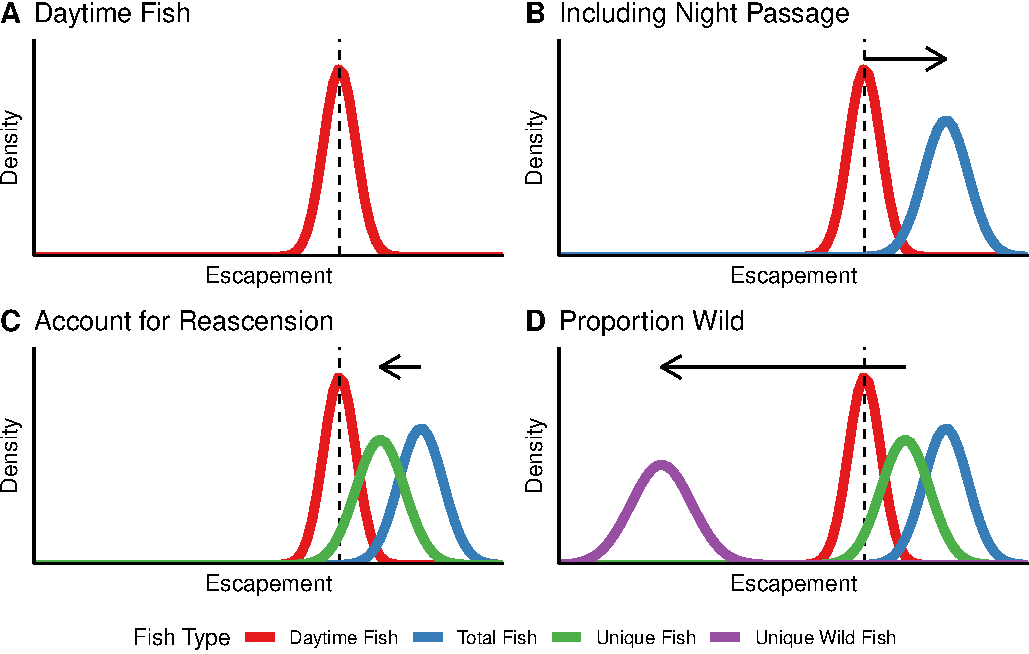
\includegraphics{../figures/stadem-examp-fig-1.pdf}
\caption{\label{fig:stadem-examp-fig}Schematic of how the STADEM model works. Panel A shows the posterior of the estimate of fish crossing the dam while the window is open (dashed line shows observed window counts). That estimate is divided by the nighttime passage rate (B). The total fish is then discounted by the reascension rate to estimate unique fish (C). Those unique fish are then multiplied by the proportion of wild fish (D), to estimate unique wild fish.}
\end{figure}

\begin{figure}
\centering
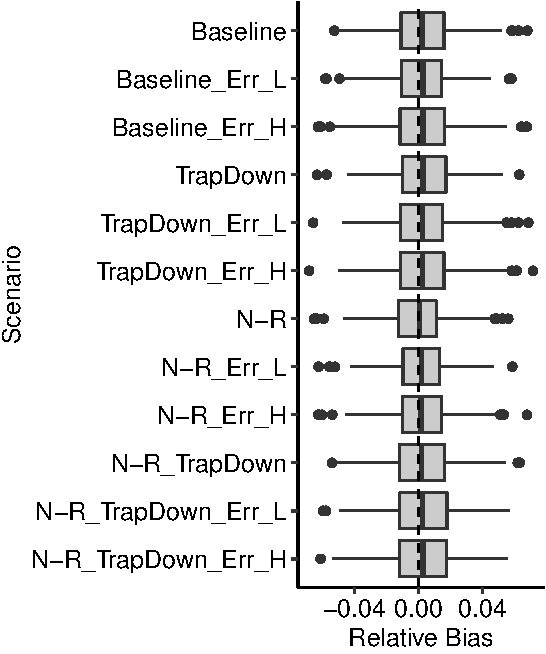
\includegraphics{../figures/rel-bias-lgd-1.pdf}
\caption{\label{fig:rel-bias-lgd}'Boxplots show relative bias of STADEM estimates for wild escapement across various scenarios. The boxes contain 50\% of the simulations, whiskers contain 95\% of the simulations, and points are outliers.}
\end{figure}

\begin{figure}
\centering
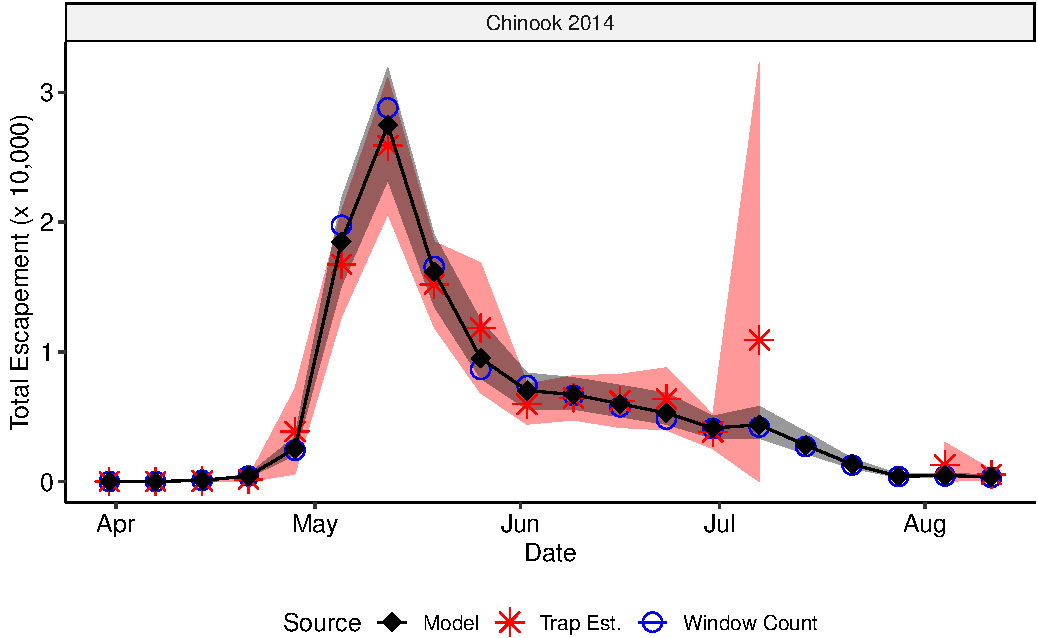
\includegraphics{../figures/jags-fit-fig-1.pdf}
\caption{\label{fig:jags-fit-fig}Time-series plot showing estimates of total escapement for Chinook in 2014, including raw window counts, window counts adjusted for night-time passage, trap estimates and STADEM estimates. Gray ribbon represents the 95\% credible interval for STADEM estimates.}
\end{figure}

\begin{figure}
\centering
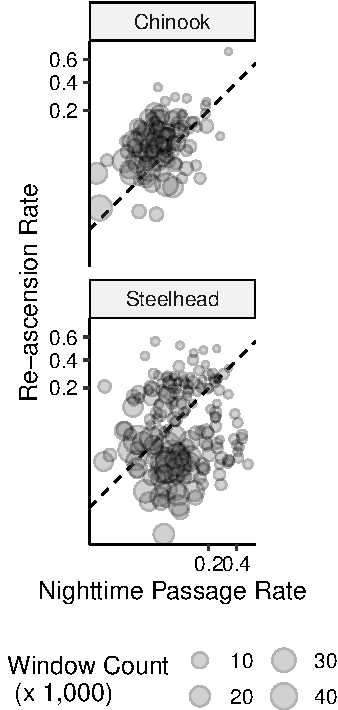
\includegraphics{../figures/night-reasc-diff-fig-1.pdf}
\caption{\label{fig:night-reasc-diff-fig}Night-time passage rate plotted against re-ascension rate, calculated from observed PIT tags for each week of spawn years 2010-2019. Colors correspond to different spawn year, while the size of each point is proportional to the window count that week. The dashed line is the 1-1 line.}
\end{figure}

\newpage

\hypertarget{append1}{%
\section{Appendix A - STADEM Model Description}\label{append1}}

\hypertarget{total-and-weekly-escapement}{%
\subsection{Total and Weekly Escapement}\label{total-and-weekly-escapement}}

Escapement at LGD is estimated by combining two independent observations, trap catches and window counts, of the true number of fish crossing the dam in a state-space model with a weekly time-step. Both are assumed to be corrupted observations of the true unknown number of fish crossing LGD each week. The log of the true number of fish crossing (\(X_t\)), is modeled as a random walk process (Shumway and Stoffer 2010).

\[
\begin{aligned}
  \ln \left( X_{t} \right) &= \ln \left( X_{t-1} \right) + e_t \\
  e_t &\sim \mathcal{N}(0, \sigma^2_X)
\end{aligned}
\]

The number of fish caught in the trap, \(Y^T_t\), for week \(t\) is modeled as a binomial process based on the unknown true trap rate that week, \(\nu_t\), and the unknown true number of fish crossing the dam that week, \(X_t\). The true trap rate is estimated from a beta distribution with previously estimated parameters, \(\hat{\alpha_t}\) and \(\hat{\beta_t}\), informed by the mark-recapture estimate of the trap rate.

\[
\begin{aligned}
  \nu_t &\sim \text{Beta} \left(\hat{\alpha_t}, \hat{\beta_t} \right) \\
  Y^T_t &\sim \text{Bin} \left( \nu_t, X_t \right) \\
\end{aligned}
\]

The estimate of the weekly trap rate is derived based on previously PIT-tagged spring/summer Chinook and steelhead who are crossing LGD that week. The fish caught in the trap that week are considered the ``mark'' group, and all the PIT tagged fish who are detected at the upper end of the LGD fish ladder that week are considered the second capture group (which includes recaptures of the the ``marked'' fish). From this data, we can estimate the total number of previoiusly PIT tagged fish crossing LGD that week, and the proportion of those that are caught in the trap is the weekly trap rate. The uncertainty in estimates of total fish is translated into uncertainty in the trap rate, and this is then summarised with a beta distribution (\(\text{Beta} \left(\hat{\alpha_t}, \hat{\beta_t} \right)\)) that becomes an input into STADEM. Although the group of previously PIT tagged fish is not assumed to be representative of the overall run, the rate at which they are caught in the trap should be the same rate that the overall run experiences.

The number of fish counted at the window, \(Y^W_t\), is modeled as a (potentially) over-dispersed negative binomial process, with an expected value of \(X_t^{day}\), the number of fish crossing the dam while the window is open. This is simply the total number of fish crossing that week, \(X_t\), multiplied by the propoortion of fish crossing while the window is open for counting, \(\theta_t\), calculated on a weekly basis. In the formula below, \(p_t\) is the proportion of fish observed at the window and \(r\) is the shape parameter. If \(r\) is estimated to be small provides evidence for over-dispersion, and as it grows very large, the negative binomial distribution behaves like a Poisson distribution.

\[
\begin{aligned}
  X_t^{day} &= X_t * \theta_t \\
  p_t &= \frac{r}{\left( r + X_t^{day} \right)} \\
  Y^W_t &\sim \text{NegBin} \left( p_t, r \right) \\
\end{aligned}
\]

Thus, the unknown true number of fish crossing LGD each week, \(X_t\), is estimated from two different data source: window counts and fish sampled in the trap. The window counts provide an estimate (with some potential observer error) of the fish crossing during daytime hours, while the fish in the trap, when expanded by the estimated true trap rate, provide an estimate of the total fish crossing that week. For weeks when we have a more precise estimate of the trap rate (i.e.~weeks when lots of previously PIT tagged fish are crossing LGD), STADEM will tend to favor the estimate of total escapement based on the trap data, whereas when that trap rate is more uncertain (e.g.~fewer PIT tagged fish to use in estimating the trap rate), STADEM will rely more on the window counts to estimate total escapement. During peak run times, when lots of fish are crossing LGD, estimates based on trap data and trap rates will be more precise, while estimates from the window counts may have more observation error due to so many fish passing the window. For weeks when the trap is down, STADEM relies exclusively on the window counts and night-time passage data, but there will be more uncertainty in the estimates.

\hypertarget{day-time-passage-and-re-ascension-rates}{%
\subsection{Day-time Passage and Re-ascension Rates}\label{day-time-passage-and-re-ascension-rates}}

There are two other processes that must be accounted for, first, the proportion of fish that cross the dam while the window is closed for counting (night-time passage rate), and the second, the proportion of fish that are crossing the dam multiple times (re-ascension rate) and therefore potentially double-counted. Both rates can be estimated from previously PIT tagged fish that are crossing the dam each week.

The proportion of fish passing the window during non-operational hours, night-time passage rate, is just the complement of the rate of fish passing during the day when the window is operating. The daytime passage rate for week \(t\), \(\theta_t\), is modeled as a random walk process and estimated from a binomial distribution based on the number of PIT tags observed to cross the dam during operational hours, \(y^{day}_t\), and the total number of PIT tags observed to cross the dam at any point that week, \(N_t\) (Shumway and Stoffer 2010).

\[
\begin{aligned}
  y^{day}_t &\sim \text{Bin} \left(\theta_t, N_t \right) \\
  \text{logit} (\theta_{t}) &= \text{logit} \left( \theta_{t-1} \right) + g_t \\
  g_t &\sim \mathcal{N}(0, \sigma^2_\theta) \\
\end{aligned}
\]

The number of total fish crossing Lower Granite differs from the number of unique fish crossing Lower Granite because some fish fall back and re-ascend the dam. These fish are potentially double-counted at the window, and have the potential to be caught in the fish trap more than once. The number of tags known to be re-ascending the dam each week, \(y^{reasc}_t\), is modeled as a binomial process based on the estimated re-ascension rate, \(\eta_t\), and the total number of tags crossing the dam that week, \(N_t\). The logit of the re-ascension rate is modeled as a random walk process similar to day-time passage (Shumway and Stoffer 2010).

\[
\begin{aligned}
  y^{reasc}_t &\sim \text{Bin} \left(\eta_t, N_t \right) \\
  \text{logit} \left( \eta_{t} \right) &= \text{logit} \left(\eta_{t-1} \right) + f_t \\
  f_t &\sim \mathcal{N}(0, \sigma^2_\eta)
\end{aligned}
\]

\hypertarget{origin-proportions}{%
\subsection{Origin Proportions}\label{origin-proportions}}

After estimating the total number of fish to have crossed Lower Granite each week, \(X_t\), the total must be further refined into the number of wild fish, \(X_{w,t}\), hatchery fish, \(X_{h,t}\) and hatchery no-clip fish, \(X_{hnc, t}\). This is done by estimating a weekly origin proportion vector, \(\omega_t\) based on the random sample of fish caught in trap that week, \(Y^T_t\). The observed number of wild, \(Y^T_{w,t}\), hatchery, \(Y^T_{h,t}\), and hatchery no-clip, \(Y^T_{hnc,t}\), fish caught in the trap that week is assumed to come from a multinomial distribution with probability vector \(\omega_t\). The log-odds ratio of the proportions in \(\omega_t\), in relation to the proportion of hatchery fish, \(\omega_{h,t}\) is modeled as a random walk, so it can change through time. This allows the proportions of wild, hatchery and hatchery no-clip fish to shift throughout the season, based on the data available from the fish trap.

\[
\begin{aligned}
  \left( Y^T_{w,t}, Y^T_{h,t}, Y^T_{hnc,t} \right) &\sim \text{Multinom} \left( \omega_t, Y^T_t \right) \\
  \omega_t &= \frac{\exp(\phi_t)}{\sum{\exp(\phi_t})} \\
  \phi_{w,t} &= \ln \left( \frac{\omega_{w,t}}{\omega_{h,t}} \right) \\
  \phi_{hnc,t} &= \ln \left( \frac{\omega_{hnc,t}}{\omega_{h,t}} \right) \\
  \phi_{h,t} &= 0 \\
  \phi_{w,t} &= \phi_{w, t-1} + d_{w,t} \\
  \phi_{hnc,t} &= \phi_{hnc, t-1} + d_{hnc,t} \\
  d_t &\sim \mathcal{N}(0, \sigma^2_\omega) \\
\end{aligned}
\]

Finally, the number of unique fish crossing Lower Granite each week, \(X_{w,t}\), is the product of the total fish crossing that week, \(X_t\) multiplied by one minus the re-ascension rate, \((1 - \eta_t)\), and the origin proportion vector, \(\omega_t\).

\[
\begin{aligned}
  \begin{bmatrix} X_{w,t} \\ X_{h,t} \\ X_{hnc,t} \end{bmatrix}
  &= X_t * (1 - \eta_t) * \begin{bmatrix} \omega_{w,t} \\ \omega_{h,t} \\ \omega_{hnc,t} \end{bmatrix}
\end{aligned}
\]

\hypertarget{model-fitting}{%
\subsection{Model Fitting}\label{model-fitting}}

The model was fit using the JAGS program (Plummer 2019), run with R software (R Core Team 2020). Uninformative priors were used for \(\sigma_X, \sigma_\eta, \sigma_\theta, \sigma_\omega\) and \(\ln(X_1)\) (Uniform(0,10)), as well as logit(\(\eta_1\)) and logit(\(\theta_1\)) (\(\mathcal{N}(0, 1000)\)), and finally \(\phi_{w,1}\) and \(\phi_{hnc,1}\) (\(\mathcal{N}(0, 100)\)).

\newpage

\hypertarget{append2}{%
\section{Appendix B - Simulation Details}\label{append2}}

To simulate fish passing a dam, an \(\mathbb{R}\) software function was developed (R Core Team 2020). The function randomly samples observations from assumed probability distribution functions (\(\mathcal{PDF}\)) with known parameters. Total unique fish, \(N\), and a vector, \(\omega\), containing the proportions of wild (\(w\)), hatchery (\(h\)) and hatchery no-clip (\(hnc\)) fish passing the dam is set to establish known ``truths'' of escapement by origin.

\[
\begin{aligned}
\left[N_{w}, N_{h}, N_{hnc} \right] &= N * \left[\omega_{w}, \omega_{h}, \omega_{hnc} \right]
\end{aligned}
\]

Escapement is then randomly divided across a set number of populations, \(n\), by randomly drawing proportions, \(\phi_{j,p}\), of origin group \(j\) in each poplulation \(p\) using a dirichlet \(\mathcal{PDF}\). The dirichlet function is parameterized from a vector, \(\eta_j\), containing 1's and 0's designating populations with origin \(j\) fish returning. \(\eta_j\) originates from a bernoulli \(\mathcal{PDF}\) and the proportion of populations with each origin, \(\tau_j\). Wild fish are assumed to be in all populations; \(\tau_w = 1.0\). The product of sampled population proportions \(\phi_{j,p}\) and fixed \(N_j\) yields a random variable of abundance for each origin in each population, \(N_{j,p}\). Summing across origin abundances then gives a random total population abundance, \(N_p\), crossing the dam.

\[
\begin{aligned}
  \left[\eta_{j,p=1},  ... , \eta_{j,p=n}\right] &\sim \text{Bern}(\tau_j) \\
  \left[\phi_{j,p=1},  ... , \phi_{j,p=n}\right] &\sim \text{Dir}(\eta_{j,p=1},  ... , \eta_{j,p=n}) \\
  N_{j,p} &= N_j * \phi_{j,p} \\
  N_p &= \sum_{j=w, h, hnc} N_{j,p}
\end{aligned}
\]

Mean arrival date, \(\bar{a}_p\), for each population returning to the dam is drawn from a normal \(\mathcal{PDF}\) with hyper-parameters \(\mu_a\) and \(\sigma^2_a\). Similarly, the variance or spread in run-timing within populations is the absolute value of random variables drawn from a normal \(\mathcal{PDF}\) with hyper-parameters \(\mu_s\) and \(\sigma^2_s\).

\[
\begin{aligned}
 \left[\bar{a}_p, ..., \bar{a}_n\right] &\sim \text{Norm}(\mu_a, \sigma^2_a) \\
 \left[s_p, ..., s_n\right] &\sim \text{Norm}(\mu_s, \sigma^2_s)
\end{aligned}
\]

After sampling the mean date of arrival and variances for each population, the date of arrival, \(a_{i,p}\), for individual fish, \(i\), within each population are drawn from a normal \(\mathcal{PDF}\) with population parameters \(\bar{a}_p\) and \(s^2_p\). This simulates a random arrival day that is similar for all fish returning to the same population, regardless of origin.

\[
\begin{aligned}
 date_{i,p} &\sim \text{Norm}(\bar{a}_p, s^2_p) \\
\end{aligned}
\]

To examine the sensitivites of models to different fish behavior and dam operational scenarios, seven addtional attributes are randomly assigned to each individual fish. Each attribute is randomly assigned a TRUE/FALSE using a bernoulli \(\mathcal{PDF}\) and a fixed probability parameter. Fish passage during the day-time (i.e., during periods of window operation) is modeled using one minus the night-time passage rate (\(1 - \nu\)). Window observations are conditioned on fish passing during the day and being observed at a set rate, \(\gamma\). Whether fish \(i\) is sampled by the adult trap is modeled on the weekly set trap rate, \(\delta_t\). The rate of previously PIT-tagged fish is determined by \(\lambda\), and their subsequent detection at the ladder PIT antenna is governed by \(\kappa\). Fallback behavior is modeled with a common rate across all populations, \(\psi\). Re-ascension occurs with probability \(\rho\), conditioned on fish \(i\) falling back. If fish \(i\) falls back and re-ascends, the entire process described above is repeated, with some time-lag between initial ascension and re-ascension that is governed by a Poisson \(\mathcal{PDF}\) with mean = 2 days. Fish may fall-back and re-ascend up to 3 times, allowing for the possibility of the same fish being counted or trapped multiple times.

\[
\begin{aligned}
  day_{i} &\sim \text{Bern}(1-\nu) \\
  window_{i|d = TRUE} &\sim \text{Bern}(\gamma) \\
  trapped_{i} &\sim \text{Bern}(\delta_t) \\
  tagged_{i} &\sim \text{Bern}(\lambda) \\
  ladder_{i|m = TRUE} &\sim \text{Bern}(\kappa) \\  
  fallback_{i} &\sim \text{Bern}(\psi) \\
  re-ascend_{i|f = TRUE} &\sim \text{Bern}(\rho)
\end{aligned}
\]

Simulation parameters for model evaluations were set to mimic typical ecapement of spring/summer Chinook to LGD with similar origin proportions, marking rates and run timing as those observed from return years 2010 - 2015. Escapement of each origin (\(N_j\)) was set at 25,000 wild, 70,000 hatchery and 5,000 hatchery no-clips spread randomly across 25 populations (\(n\)). Of the 25 populations, each had a 1.0 probability of containing wild fish, 0.50 probability of having hatchery fish and 0.15 probability of receiving hatchery no-clip (\(\tau_j\)); resulting in an expected 25 wild, 12.5 hatchery and 3.75 hatchery no-clip populations. Mean arrival dates and variability were estimated from PIT-tag detection data queried from the Columbia Basin Research Data Access in Real Time (\href{http://www.cbr.washington.edu/dart/query/pit_adult_window}{DART}) website and organized by release subbasin. Mean arrival date across all subbasins and 2010 - 2015 return years was June \(19^{th}\) (\(\mu_a = 171\)) with a standard deviation of 13 days (\(\sigma_a\)). While the observed spread (i.e., variance) of arrival dates within subbasins was determined to have a mean (\(\mu_s\)) of 22 days and a standard deviation of 7 days (\(\sigma_s\)).

For the specific simulated scenarios, we were interested in STADEM model estimates of origin specific escapment from the combinations of two seperate trapping rates, two fallback, re-ascension and night-passage combinations and three window count error rates; resulting in twelve different scenarios. First, trapping rates were set static at 0.15 across all weeks for six scenarios to mimic an optimium trap operation for an expected return of 25,000 wild fish (i.e., trap \(\approx\) 4,000 wild fish). For the remaining six scenarios, trapping rates for weeks 30, 31 and 32 (i.e., July \(22^{nd}\) to August \(11^{th}\)) were changed to 0.00 to test STADEM sensitivities to potential trap shut downs similar to those observed in 2013, 2014 and 2015 (Ogden 2014, 2016b, 2016a). To simulate and control the number of re-ascending and night-time passing fish to model response, we altered fallback and night-time passage rates while holding the re-ascension rate constant at \(\rho = 1.0\). Altering fallback rates and holding re-ascension constant allowed for a more simple control of the number of fish re-ascending; because the number of re-ascending fish is a function of the number of fallbacks and the re-ascension rate. Six scenarios had equal rates of fallback and night-time passage set at \(\psi = \nu = 0.06\) (Boggs et al. 2004) which means other estimator assumptions (Schrader et al. 2013). The other six scenarios set fallback at \(\psi = 0.10\) and night-time passage at \(\nu = 0.05\) to create a 5.0\% positive bias of unique fish at the window. A potential 5.0\% weekly bias was determined from PIT-tag data and within the range of observed weekly difference for return years 2010 - 2015 (Figure \ref{fig:night-reasc-diff-fig}). Finally, we desired to test the sensitivites of STADEM to potential rates of window count error; 0\%, 5\% and 10\% (Hatch et al. 1994). Error at the window was simulated as unbiased (i.e., expect varying high and low counts to cancel each other) and is introduced to the sum of daily window counts using a normal \(\mathcal{PDF}\).

\end{document}
